% pdflatex HLA.tex
\documentclass[12pt]{article}

\usepackage{fullpage}
\usepackage{multicol, multirow}
\usepackage{tabularx}
\usepackage{graphicx}
\usepackage{ulem}
\usepackage[utf8]{inputenc}
\usepackage[russian]{babel}

\begin{document}

\section*{Высокоуровневая архитектура}

\subsection*{Концепция}
% Короткий рассказ о системе

Программа интернет-мессенджер для социальной сети <<Вконтакте>>. Программа позволит отправлять и принимать текстовые сообщения, управлять списком друзей.

\subsection*{Физическая архитектура}
% Диаграмма
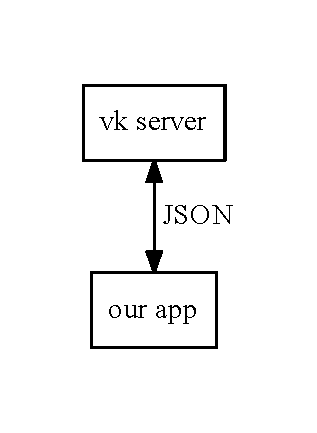
\includegraphics{./diag/phys.pdf}

\subsection*{Логическая архитектура}
% Описание модулей и их взаимодействия, диаграмма
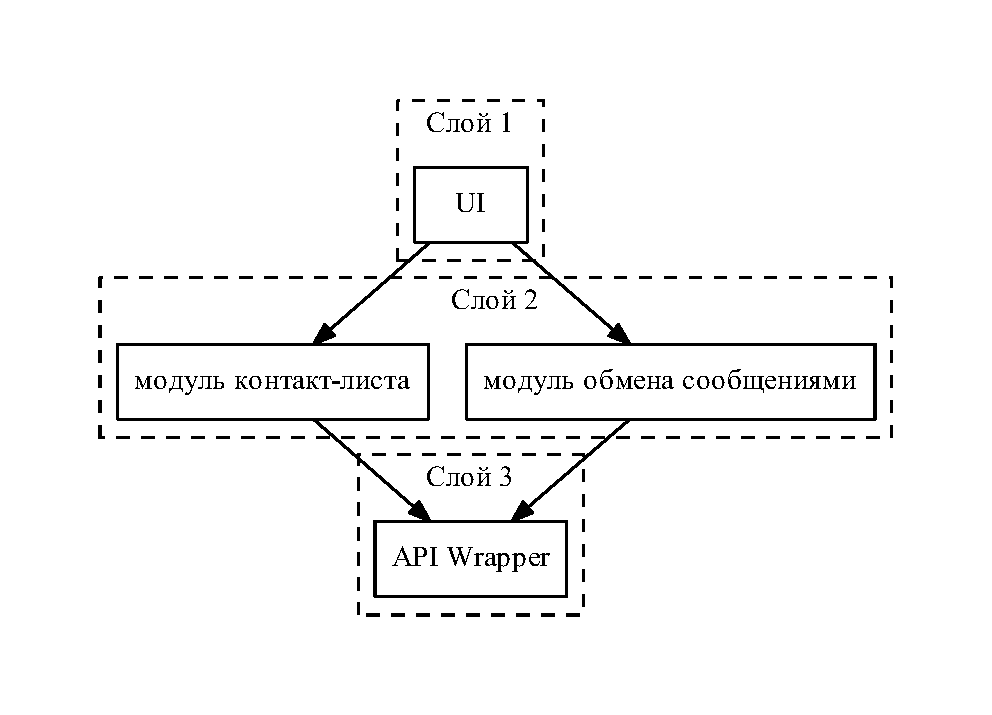
\includegraphics{./diag/logic.pdf}

\subsection*{Нефункциональные требования}
% Требования, накладывающиеся на какие-то свойства системы

%\subsubsection*{Производительность}

\subsubsection*{Надежность}
Переподключение при разрыве связи. Перепосылка недоставленных сообщений.

\subsubsection*{Сопровождаемость}
Самодокументируемый код, комментарии к неочевидным моментам.

\subsubsection*{Требования к ресурсам}

\subsubsection*{Пользовательский интерфейс}
Англоязычный пользовательский интерфейс. Интуитивность и минималистичность интерфейса.

\subsubsection*{Операционное окружение}
Кроссплатформенность.

\subsubsection*{Безопасность}
Шифрование сохраненного пароля пользователя.
Разграничение прав при хранении истории сообщений.

\subsection*{Компоненты и инструменты}
% 
\begin{enumerate}
\item Python 2.7.2
\item PyQt 4.10.3
\item vkontakte 1.3.2 (vk.com (aka vkontakte.ru) API wrapper)
\end{enumerate}

\end{document}

